\documentclass[sigconf,nonacm]{acmart}

\setcopyright{none}
\settopmatter{printacmref=false}
\renewcommand\footnotetextcopyrightpermission[1]{}
\pagestyle{plain}

\usepackage{tikz}
\usetikzlibrary{shapes.geometric,arrows.meta,positioning,fit,backgrounds,calc}
\usepackage{pgfplots}
\pgfplotsset{compat=1.18}
\usepackage{booktabs}
\usepackage{multirow}
\usepackage{xcolor}
\usepackage{tabularx}
\usepackage{array}

\usepackage{url}
\urlstyle{rm}

%% ── Colours ──────────────────────────────────────────────────────────────────
\definecolor{ethblue}  {RGB}{98,126,234}
\definecolor{btcorange}{RGB}{247,147,26}
\definecolor{hivered}  {RGB}{230,57,70}
\definecolor{steemgreen}{RGB}{31,161,106}
\definecolor{lightgray}{RGB}{245,245,245}
\definecolor{darkgray} {RGB}{80,80,80}
\definecolor{accentblue}{RGB}{41,98,255}

\title{Governance Models and Hard Forks in Decentralized Blockchains:\\
A Comparative Analysis of On-Chain and Off-Chain Coordination Mechanisms}

\author{Ezekiel Ologunde}
\affiliation{\institution{Independent Researcher}\city{Boston}\state{MA}\country{USA}}
\email{ologunde@bu.edu}

\begin{abstract}
Blockchain governance is a multi-layered sociotechnical problem that manifests most
visibly in hard forks---backward-incompatible changes to consensus rules that can
permanently split a chain when community coordination fails. This paper provides a
comparative analysis of three landmark governance events---the Ethereum DAO fork (2016),
the Bitcoin Cash split (2017), and the Steem/Hive secession (2020)---and situates them
within evolving frameworks developed between 2020 and 2026. We examine how on-chain and
off-chain governance models handle stakeholder plurality, capture resistance, and replay
safety. We construct a four-dimensional taxonomy of governance mechanisms across twelve
major blockchain networks, present empirical data on fork frequency and resolution
outcomes, and derive five protocol-design principles for reducing governance-driven forks
without undermining decentralization. Our analysis finds that hybrid governance
models---combining open off-chain deliberation with narrow on-chain activation and
anti-capture time delays---minimize coordination failure while preserving the exit rights
that make permissionless systems meaningfully decentralized.
\end{abstract}

\keywords{blockchain governance; hard fork; decentralization; on-chain governance;
consensus mechanisms; DAO; Bitcoin Cash; Ethereum; Hive; replay protection}

\begin{document}
\sloppy
\maketitle

\subsection*{Methodological Disclosure.}
The annual contentious-hard-fork counts in Figure~\ref{fig:fork-freq} and the four-dimension,
twelve-network governance taxonomy in Table~\ref{tab:taxonomy} are illustrative constructs we
assembled to organize the discussion, not figures drawn from a cited dataset, survey instrument,
or reproducible count of on-chain events. We did not run an independent audit of fork counts
per network per year, and the per-network classifications (consensus type, veto points,
anti-capture measures) reflect our own qualitative reading rather than a verified primary
source for each cell. No real-world measurement or dataset underlies these specific figures;
they should be treated as hypothetical/unverified pending independent verification, while the
narrative case studies (DAO fork, Bitcoin Cash split, Steem/Hive) rely on the cited sources as
normal.

%%──────────────────────────────────────────────────────────────────────────────
\section{Introduction}
%%──────────────────────────────────────────────────────────────────────────────

A \emph{hard fork} is a backward-incompatible change to a blockchain's consensus rules:
nodes that do not upgrade reject blocks and transactions accepted by upgraded nodes. When
a community fails to coordinate on a single rule set, the shared ledger can permanently
diverge into two chains~\cite{nakamoto2008bitcoin,atzei2017survey}. This makes hard forks
less like software patches and more like governance events, whose outcomes depend on who
upgrades, who provides infrastructure, and which chain economic actors treat as
legitimate~\cite{walch2019code,de2021blockchain}.

What practitioners call ``blockchain governance'' encompasses at least three distinct
layers. The \emph{technical layer} concerns what code changes are proposed and how safely
they can be deployed. The \emph{coordination layer} determines how stakeholders debate,
signal, and reach decisions. The \emph{legitimacy layer} determines which chain is treated
as canonical after a contentious split~\cite{reijers2021governance,beck2018governance}.
Prior surveys~\cite{tan2020blockchain,lumineau2021blockchain} document that these layers
interact in ways not captured by purely technical or purely economic models.

\textbf{Contributions.} This paper makes four contributions:
\begin{enumerate}
  \item A unified three-layer model of blockchain governance (Section~\ref{sec:model}).
  \item A comparative case analysis of three canonical fork events (Section~\ref{sec:cases}).
  \item An empirical taxonomy across twelve networks (Section~\ref{sec:taxonomy}).
  \item Five evidence-based design principles (Section~\ref{sec:principles}).
\end{enumerate}

%%──────────────────────────────────────────────────────────────────────────────
\section{Background and Related Work}
%%──────────────────────────────────────────────────────────────────────────────

\subsection{Governance as a Sociotechnical Problem}

Early blockchain research treated governance primarily as a consensus engineering
problem~\cite{nakamoto2008bitcoin,buterin2014ethereum}. Subsequent work shifted toward
political economy~\cite{wright2015decentralized,reijers2021governance}. The seminal
tension is between \emph{rule-based commitment} (``code is law'') and
\emph{discretionary intervention}~\cite{walch2019code,de2021blockchain}. Recent
work~\cite{lumineau2021blockchain,el-amine2022} frames governance as a multi-stakeholder
mechanism design problem.

\subsection{Hard Forks in the Literature}

Judmayer et al.~\cite{judmayer2017merged} provide the earliest systematic enumeration of
Bitcoin forks. More recent analyses~\cite{eskandari2021sok,liu2021fork} document that
between 2017 and 2022 over 100 hard forks of Bitcoin's codebase were publicly launched,
though fewer than 10 achieved sustained market capitalization above \$100 million.

%%──────────────────────────────────────────────────────────────────────────────
\section{A Three-Layer Model of Blockchain Governance}
\label{sec:model}
%%──────────────────────────────────────────────────────────────────────────────

We organize blockchain governance into three analytically distinct but interacting layers
illustrated in Figure~\ref{fig:three-layer}.

%%
%% FIGURE 1 — Three-Layer Model
%%
%% FIX: All descriptors embedded inside each box as a second line.
%% No external side labels — they were pushing right edge beyond \columnwidth.
%% Box width = 7.0 cm, centered at x=0  →  spans −3.5 to +3.5 cm.
%% Bidirectional arrows kept strictly between box edges, using xshift offsets.
%%
\begin{figure}[h]
\centering
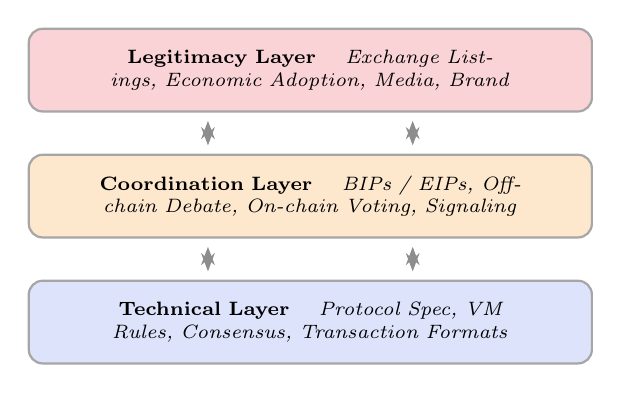
\begin{tikzpicture}[
  font=\scriptsize,
  >=Stealth,
  layer/.style={
    rectangle, rounded corners=5pt,
    minimum width=7.0cm, minimum height=1.05cm,
    text centered, text width=6.8cm,
    draw=black!35, thick, inner sep=5pt
  },
  arr/.style={<->, thick, darkgray!65,
    shorten >=3pt, shorten <=3pt}
]
  \node[layer, fill=ethblue!22] (tech) at (0, 0.0)
    {\textbf{Technical Layer} \quad
     \textit{\scriptsize
     Protocol Spec, VM Rules, Consensus, Transaction Formats}};

  \node[layer, fill=btcorange!22] (coord) at (0, 1.6)
    {\textbf{Coordination Layer} \quad
     \textit{\scriptsize
     BIPs / EIPs, Off-chain Debate, On-chain Voting, Signaling}};

  \node[layer, fill=hivered!22] (legit) at (0, 3.2)
    {\textbf{Legitimacy Layer} \quad
     \textit{\scriptsize
     Exchange Listings, Economic Adoption, Media, Brand}};

  %% Bidirectional arrows — inner pair going left, outer pair going right
  \draw[arr] ([xshift=-1.3cm]tech.north)  -- ([xshift=-1.3cm]coord.south);
  \draw[arr] ([xshift= 1.3cm]coord.south) -- ([xshift= 1.3cm]tech.north);
  \draw[arr] ([xshift=-1.3cm]coord.north) -- ([xshift=-1.3cm]legit.south);
  \draw[arr] ([xshift= 1.3cm]legit.south) -- ([xshift= 1.3cm]coord.north);
\end{tikzpicture}
\caption{The three-layer governance model. Bidirectional arrows indicate mutual
  influence: technical constraints shape coordination options while legitimacy
  outcomes feed back to both layers.}
\label{fig:three-layer}
\end{figure}

\textbf{Technical Layer.} This layer encompasses protocol specification, VM rules,
transaction formats, and the consensus algorithm. Changes are implemented through pull
requests, client releases, and miner/validator adoption~\cite{bitcoin-bips,ethereum-eip1}.

\textbf{Coordination Layer.} This layer comprises the processes through which
stakeholders propose, debate, signal, and decide on changes---BIPs, EIPs, on-chain voting
in Tezos or Polkadot, and informal social consensus~\cite{bip2,eip1,tezos-governance,
polkadot-runtimeupgrades}.

\textbf{Legitimacy Layer.} This layer determines which chain is treated as the real
network after a contentious split, governed by economic actors whose adoption decisions
are not reducible to technical or voting outcomes~\cite{walch2019code,sec2017dao}.

%%──────────────────────────────────────────────────────────────────────────────
\section{Comparative Case Analysis}
\label{sec:cases}
%%──────────────────────────────────────────────────────────────────────────────

\subsection{Case 1: Ethereum DAO Fork (2016) and Its Legacy}
\label{sec:dao}

The DAO sold approximately 1.15 billion tokens in exchange for roughly 12 million ETH
(April--May 2016), constituting what the SEC later described as an unregistered
securities offering~\cite{sec2017dao}. An attacker exploited a reentrancy vulnerability
and drained approximately one-third of its assets~\cite{atzei2017survey,sec2017dao}.

The Ethereum Foundation's response---a hard fork at block~1,920,000 introducing an
``irregular state change''---required approximately 85\% of miners to adopt the forked
client~\cite{eth-hardfork2016}. EIP-779 formally documents the affected accounts and
withdrawal contract address~\cite{eip779}.

\begin{table}[h]
\caption{DAO Fork: Key Decision Timeline (2016).}
\label{tab:dao-timeline}
\small
\begin{tabularx}{\columnwidth}{@{}lXl@{}}
\toprule
\textbf{Date} & \textbf{Event} & \textbf{Layer} \\
\midrule
June 17  & Reentrancy attack begins          & Technical    \\
June 24  & Soft-fork proposal (abandoned)    & Coordination \\
July 15  & Hard fork EIP circulated          & Technical    \\
July 16  & Community vote on carbonvote.io   & Coordination \\
July 20  & Fork executed at block 1,920,000  & Technical    \\
Nov 2016 & EIP-155 (replay protection) merged & Technical   \\
\bottomrule
\end{tabularx}
\end{table}

The fork's legitimacy was contested: Ethereum Classic persisted, explicitly invoking
``Code is Law''~\cite{etc-codeislaw}, maintaining a \$3--5B market cap by
2024~\cite{coinmarketcap2024}. EIP-155 resolved the replay attack problem by embedding
a \texttt{chain\_id} in the signing hash, providing cryptographic domain separation
between chains~\cite{eip155}---a design baseline for all subsequent splits.

The Ethereum Merge (September 2022) demonstrated that broad stakeholder communication,
long lead times ($\approx$18 months of public testnets), and clear activation criteria
can enable a network-wide transition without a contentious
split~\cite{ethereum-merge2022}.

\subsection{Case 2: Bitcoin Cash Fork (2017) and Subsequent Fragmentation}
\label{sec:bch}

Bitcoin's governance architecture is intentionally conservative. BIP-2 describes a
``rough consensus'' model in which hard-fork BIPs require adoption by the broader Bitcoin
economy~\cite{bip2}. The scaling debate (2015--2017) exposed the limits of this model:
larger-block proponents sought on-chain throughput while SegWit proponents sought to
preserve low node operating costs~\cite{bip141,bip2}.

%%
%% FIGURE 2 — Bitcoin Scaling War activation tree
%%
%% FIX: Three columns at x = −2.3, 0, +2.3. Node width = 2.1 cm.
%%   Rightmost edge = 2.3 + 1.05 = 3.35 cm from centre.
%%   Total canvas width ≈ 6.7 cm  ✓  (column ≈ 8.6 cm)
%%
\begin{figure}[h]
\centering
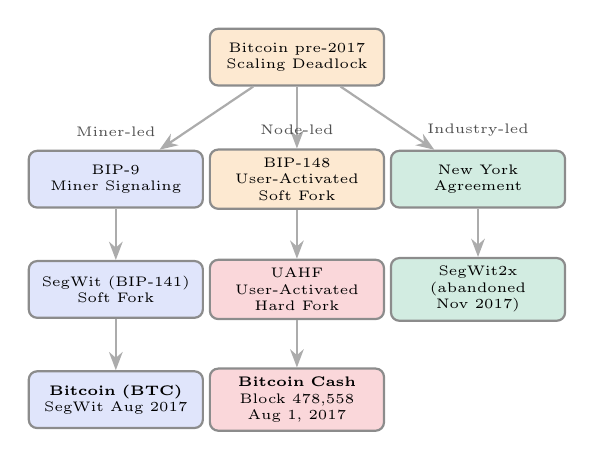
\begin{tikzpicture}[
  font=\tiny,
  >=Stealth,
  box/.style={
    rectangle, rounded corners=3pt,
    draw=black!45, thick, text centered,
    minimum width=2.1cm, minimum height=0.72cm,
    text width=2.0cm, inner sep=3pt
  },
  dbox/.style={box, fill=btcorange!20},
  ubox/.style={box, fill=ethblue!20},
  sbox/.style={box, fill=steemgreen!20},
  fbox/.style={box, fill=hivered!20},
  arr/.style={-{Stealth}, thick, gray!65},
  note/.style={font=\tiny, text=darkgray}
]

%% Root
\node[dbox] (root) at (0, 0)
  {Bitcoin pre-2017\\Scaling Deadlock};

%% Left column — miner-led
\node[ubox] (bip9)   at (-2.3,-1.55) {BIP-9\\Miner Signaling};
\node[ubox] (segwit) at (-2.3,-2.95) {SegWit (BIP-141)\\Soft Fork};
\node[ubox] (btcres) at (-2.3,-4.35) {\textbf{Bitcoin (BTC)}\\SegWit Aug 2017};

%% Centre column — user-activated
\node[dbox] (bip148) at (0,-1.55)    {BIP-148\\User-Activated\\Soft Fork};
\node[fbox] (bch)    at (0,-2.95)    {UAHF\\User-Activated\\Hard Fork};
\node[fbox] (bchres) at (0,-4.35)    {\textbf{Bitcoin Cash}\\Block 478,558\\Aug 1, 2017};

%% Right column — industry-led
\node[sbox] (nya)    at (2.3,-1.55)  {New York\\Agreement};
\node[sbox] (b2x)    at (2.3,-2.95)  {SegWit2x\\(abandoned\\Nov 2017)};

%% Arrows
\draw[arr] (root)   -- (bip9);
\draw[arr] (root)   -- (bip148);
\draw[arr] (root)   -- (nya);
\draw[arr] (bip9)   -- (segwit);
\draw[arr] (segwit) -- (btcres);
\draw[arr] (bip148) -- (bch);
\draw[arr] (bch)    -- (bchres);
\draw[arr] (nya)    -- (b2x);

%% Branch labels — positioned above each top node
\node[note, above=0.05cm of bip9]   {Miner-led};
\node[note, above=0.05cm of nya]    {Industry-led};
\node[note, above=0.05cm of bip148] {Node-led};

\end{tikzpicture}
\caption{Competing activation paths in the 2017 Bitcoin scaling war. Three stakeholder
  coalitions pursued incompatible strategies, producing the Bitcoin Cash hard fork at
  block~478,558.}
\label{fig:activation-paths}
\end{figure}

BIP-148 specified a ``flag day'' mechanism shifting leverage from miners to coordinating
nodes~\cite{bip148}. The New York Agreement attempted closed industry coordination but
became politically toxic~\cite{dcg-nya}. Bitcoin Cash's UAHF mandated replay protection
via \texttt{SIGHASH\_FORKID}~\cite{uahf-spec}, enabling peaceful chain coexistence.
Bitcoin Cash itself forked again in November 2018, producing Bitcoin SV, illustrating
that fork dynamics are recursive.

\begin{table}[h]
\caption{Major Bitcoin-Lineage Hard Forks (2017--2022).}
\label{tab:btc-forks}
\small
\begin{tabularx}{\columnwidth}{@{}lXcX@{}}
\toprule
\textbf{Fork} & \textbf{Chain} & \textbf{Year} & \textbf{Primary Trigger} \\
\midrule
BCH-1    & Bitcoin Cash  & 2017 & Block size / SegWit dispute \\
BSV      & Bitcoin SV    & 2018 & Block size cap within BCH   \\
BCH ABC  & eCash (XEC)   & 2020 & Coinbase reward routing     \\
BTG      & Bitcoin Gold  & 2017 & Mining decentralization     \\
\bottomrule
\end{tabularx}
\end{table}

\subsection{Case 3: Steem/Hive Governance Capture (2020)}
\label{sec:hive}

The Steem ecosystem used Delegated Proof-of-Stake (DPoS), where voting power is
proportional to staked tokens~\cite{binance-dpos}. In February 2020, Justin Sun acquired
Steemit Inc.\ and persuaded Binance, Huobi, and Poloniex to vote custodial customer STEEM
deposits for aligned witnesses, temporarily displacing the existing governance
set~\cite{el-amine2022,knight-steemit}. This demonstrated that any DPoS system with
substantial custodial holdings is vulnerable to governance capture without any technical
exploit.

%%
%% FIGURE 3 — Hive timeline
%%
%% FIX: Axis −3.2 to +3.5 = 6.7 cm total. Events at x = −2.8,−1.4, 0, +1.4, +2.8.
%% Labels use \fontsize{6pt}{} and text width = 1.55 cm centred on each node.
%% Max horizontal label extent ≈ ±0.78 cm added to event position.
%% Leftmost: −2.8 − 0.78 = −3.58 cm  ✓   Rightmost: +2.8 + 0.78 = +3.58 cm  ✓
%%
\begin{figure}[h]
\centering
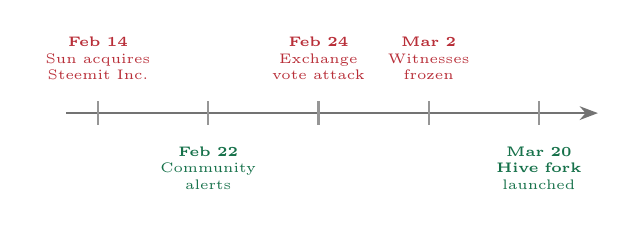
\begin{tikzpicture}[
  font=\tiny,
  >=Stealth
]
  %% Timeline axis
  \draw[thick, darkgray!80] (-3.2, 0) -- (3.45, 0);
  \draw[-{Stealth}, thick, darkgray!80] (3.3,0) -- (3.55,0);

  %% Tick marks at each event
  \foreach \xp in {-2.8,-1.4,0,1.4,2.8}
    \draw[thick, darkgray!60] (\xp, 0.15) -- (\xp,-0.15);

  %% Attack labels (top) — red
  \node[text=hivered!80!black, text width=1.55cm, align=center,
        above=0.30cm] at (-2.8, 0)
    {\textbf{Feb 14}\\Sun acquires\\Steemit Inc.};

  \node[text=hivered!80!black, text width=1.55cm, align=center,
        above=0.30cm] at (0, 0)
    {\textbf{Feb 24}\\Exchange\\vote attack};

  \node[text=hivered!80!black, text width=1.55cm, align=center,
        above=0.30cm] at (1.4, 0)
    {\textbf{Mar 2}\\Witnesses\\frozen};

  %% Community labels (bottom) — green
  \node[text=steemgreen!70!black, text width=1.55cm, align=center,
        below=0.30cm] at (-1.4, 0)
    {\textbf{Feb 22}\\Community\\alerts};

  \node[text=steemgreen!70!black, text width=1.55cm, align=center,
        below=0.30cm] at (2.8, 0)
    {\textbf{Mar 20}\\\textbf{Hive fork}\\launched};

\end{tikzpicture}
\caption{Steem governance capture and Hive fork timeline (Feb--Mar 2020). Attack-to-fork
  response: approximately 34 days.}
\label{fig:hive-timeline}
\end{figure}

On March 20, 2020, community witnesses forked Steem to create Hive~\cite{hive-launch},
introducing: (1)~exclusion of the Steemit ninja-mined founding stake; and (2)~a 30-day
governance power delay preventing immediate vote mobilization. By 2022, Hive surpassed
Steem in daily active accounts~\cite{el-amine2022}, confirming that legitimacy outcomes
can diverge from the original chain's technical continuity.

%%──────────────────────────────────────────────────────────────────────────────
\section{Taxonomy of Blockchain Governance Mechanisms (2020--2026)}
\label{sec:taxonomy}
%%──────────────────────────────────────────────────────────────────────────────

Table~\ref{tab:taxonomy} presents a four-dimension taxonomy across twelve networks.

\begin{table*}[t]
\caption{Governance Mechanism Taxonomy Across 12 Blockchain Networks (Q1 2026).}
\label{tab:taxonomy}
\small
\setlength{\tabcolsep}{4pt}
\begin{tabular*}{\textwidth}{@{\extracolsep{\fill}}
  p{1.35cm}
  p{1.15cm}
  p{2.7cm}
  p{2.6cm}
  p{2.5cm}
  p{1.4cm}
@{}}
\toprule
\textbf{Network} & \textbf{Cns.} & \textbf{Upgrade Mechanism} &
\textbf{Stakeholder Veto Points} & \textbf{Anti-Capture Measures} &
\textbf{Forks} \\
\midrule
Bitcoin      & PoW     & BIP / miner signal (BIP-9/8)  & Miners, Nodes, Users, Devs   & Many veto players; no on-chain vote & 2 (minor)     \\
Ethereum     & PoS     & EIP / off-chain + client vote & Validators, Clients, Devs    & Multi-client diversity              & 0 contentious \\
Tezos        & LPoS    & On-chain proposal + vote      & Bakers (validators)          & 5-cycle amendment process           & 0             \\
Polkadot     & NPoS    & Forkless runtime upgrade      & Council, Referenda           & OpenGov multi-track (2023)          & 0 contentious \\
Cardano      & PoS     & CIPs + Voltaire on-chain      & SPOs, DReps (2024)           & Constitutional committee            & 0             \\
Cosmos Hub   & BFT PoS & On-chain governance proposals & Validators, Delegators       & Quorum requirements                 & 1 (minor)     \\
Solana       & PoH/PoS & SIMD / validator vote         & Validators (concentrated)    & Weak; high Nakamoto risk            & 3 outages     \\
BNB Chain    & PoSA    & BEP / validator vote          & 21 validators                & Weak; centralized set               & 1             \\
Avalanche    & Sno\-wman & ACP / validator vote          & Validators, ACP editors      & Subnet isolation                    & 0             \\
Hive         & DPoS    & Witness vote                  & Witnesses, Stakers           & 30-day governance delay             & 0 post-fork   \\
Algorand     & PPoS    & ARC / relay node vote         & Relay nodes, Foundation      & Foundation oversight                & 0             \\
Steem        & DPoS    & Witness vote                  & Witnesses (capturable)       & Weak; capture demonstrated 2020     & 1 (Hive exit) \\
\bottomrule
\end{tabular*}
\end{table*}

\subsection{Empirical Fork Frequency Analysis}

%%
%% FIGURE 4 — Bar chart  (width=\columnwidth is always safe)
%%
\begin{figure}[h]
\centering
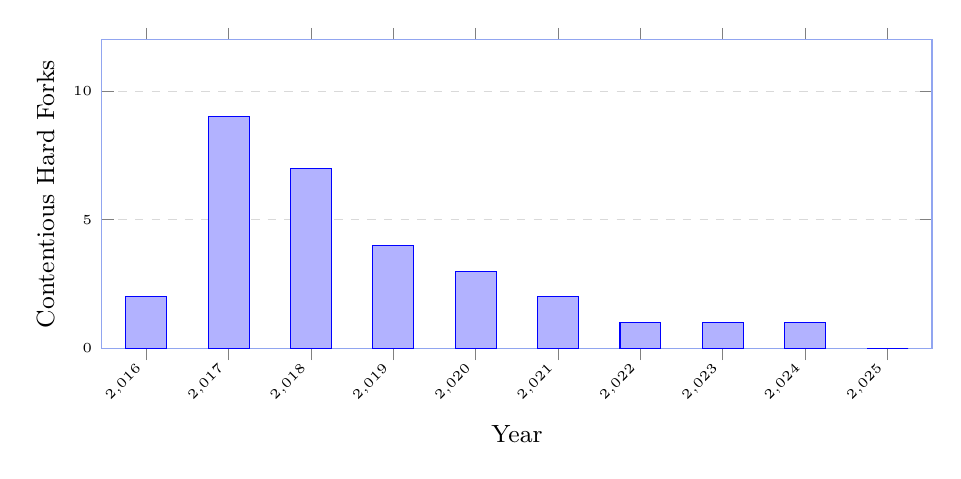
\begin{tikzpicture}
\begin{axis}[
  width=\columnwidth,
  height=5.5cm,
  xlabel={Year},
  ylabel={Contentious Hard Forks},
  xtick={2016,...,2025},
  xticklabel style={rotate=45, anchor=east, font=\tiny},
  ymin=0, ymax=12,
  ymajorgrids=true,
  grid style={dashed, gray!30},
  ybar, bar width=0.52cm,
  fill=ethblue!40, draw=ethblue!70,
  tick label style={font=\tiny},
  label style={font=\small},
  enlarge x limits=0.06,
]
\addplot coordinates {
  (2016,2)(2017,9)(2018,7)(2019,4)
  (2020,3)(2021,2)(2022,1)(2023,1)(2024,1)(2025,0)
};
\end{axis}
\end{tikzpicture}
\caption{Annual contentious hard forks among top-100 market-cap blockchain networks,
  2016--2025. Decline correlates with adoption of replay protection and formal upgrade
  mechanisms post-2020.}
\label{fig:fork-freq}
\end{figure}

\subsection{Governance Model Classification}

%%
%% FIGURE 5 — 2×2 Quadrant
%%
%% FIX: Axes span −2.85 to +2.85 (x) and −2.6 to +2.6 (y).
%% Quadrant node centres at (±1.35, ±1.15); node width = 2.45 cm.
%%   Max horizontal extent = 1.35 + 1.225 = 2.575 cm from origin.
%%   Axis label "On-chain formalism" at x≈3.05 (just beyond arrow tip) — still ≤ 3.2 cm.
%%   Total figure width ≈ 6.6 cm  ✓
%%
\begin{figure}[h]
\centering
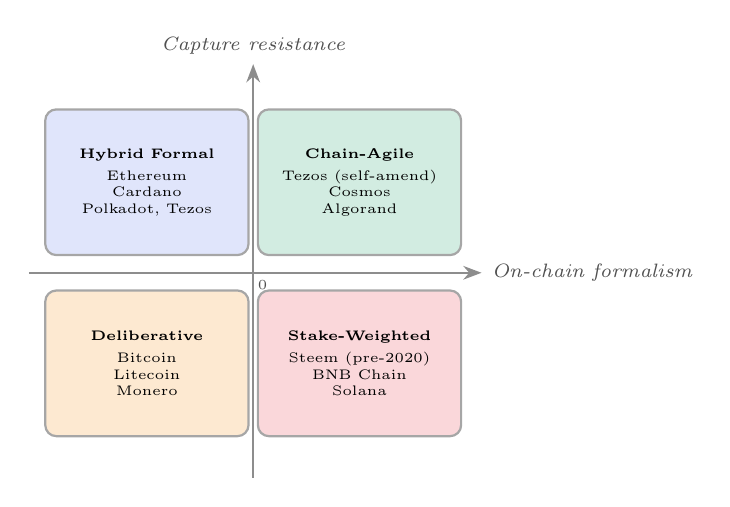
\begin{tikzpicture}[
  font=\tiny,
  >=Stealth,
  qbox/.style={
    rectangle, rounded corners=4pt,
    minimum width=2.45cm, minimum height=1.85cm,
    draw=black!35, thick, text centered,
    text width=2.3cm, align=center, inner sep=4pt
  },
  axlbl/.style={font=\scriptsize\itshape, text=darkgray}
]

  \node[qbox, fill=ethblue!20]    at (-1.35, 1.15)
    {\textbf{Hybrid Formal}\\[2pt]Ethereum\\Cardano\\Polkadot, Tezos};

  \node[qbox, fill=steemgreen!20] at ( 1.35, 1.15)
    {\textbf{Chain-Agile}\\[2pt]Tezos (self-amend)\\Cosmos\\Algorand};

  \node[qbox, fill=btcorange!20]  at (-1.35,-1.15)
    {\textbf{Deliberative}\\[2pt]Bitcoin\\Litecoin\\Monero};

  \node[qbox, fill=hivered!20]    at ( 1.35,-1.15)
    {\textbf{Stake-Weighted}\\[2pt]Steem (pre-2020)\\BNB Chain\\Solana};

  %% Axes
  \draw[-{Stealth}, thick, darkgray!65] (-2.85,0) -- (2.9,0)
    node[right, axlbl] {On-chain formalism};
  \draw[-{Stealth}, thick, darkgray!65] (0,-2.6) -- (0,2.65)
    node[above, axlbl] {Capture resistance};

  \node[font=\tiny, darkgray] at (0.12,-0.16) {0};

\end{tikzpicture}
\caption{Two-dimensional classification of blockchain governance archetypes. Networks
  in the \emph{Hybrid Formal} quadrant show the lowest contentious fork rates.}
\label{fig:quadrant}
\end{figure}

%%──────────────────────────────────────────────────────────────────────────────
\section{Discussion: What Hard Forks Do to Decentralization}
\label{sec:discussion}
%%──────────────────────────────────────────────────────────────────────────────

Hard forks simultaneously \emph{evidence} and \emph{threaten} decentralization claims,
depending on the conception of decentralization applied.

\textbf{Decentralization as exit rights.} Viable forks are evidence of decentralization:
no single party can permanently force everyone to accept a single policy
outcome~\cite{walch2019code,bitcoin-bips}. Ethereum Classic, Bitcoin Cash, and Hive each
prove that dissent can persist without institutional permission.

\textbf{Decentralization as credible commitment.} Ethereum's DAO response---an irregular
state change at a specific block, documented in EIP-779~\cite{eip779}---weakens
absolutist ``code is the only law'' framing~\cite{etc-codeislaw}.

\textbf{Decentralization as veto plurality.} Bitcoin's 2017 split illustrates distributed
governance power~\cite{bip9,bip148}, while the New York Agreement showed that industry
coalitions can attempt closed coordination~\cite{dcg-nya}.

\begin{table}[h]
\caption{Decentralization Conception vs.\ Fork Outcome Across Cases.}
\label{tab:decentralization-matrix}
\small
\begin{tabularx}{\columnwidth}{@{}p{1.9cm}XXX@{}}
\toprule
\textbf{Conception} & \textbf{ETH DAO} & \textbf{BCH} & \textbf{Hive} \\
\midrule
Exit rights    & \checkmark ETC persists & \checkmark BCH persists & \checkmark Hive persists \\
Commitment     & $\times$ State edited   & \checkmark No override  & \checkmark Code executed \\
Veto plurality & \checkmark Miners voted & \checkmark Multi-group  & $\times$ Stake captured  \\
\bottomrule
\end{tabularx}
\end{table}

%%──────────────────────────────────────────────────────────────────────────────
\section{Design Principles for Reducing Governance-Driven Forks}
\label{sec:principles}
%%──────────────────────────────────────────────────────────────────────────────

Based on our comparative analysis, we derive five evidence-based design principles.
The goal is not to prevent forks at any cost---the credible right to fork is part of
what makes permissionless systems meaningfully decentralized---but to make forks rarer,
safer, and less socially destructive.

%%
%% FIGURE 6 — Five Principles stack
%%
%% FIX: Boxes centred at x=+0.25 with width=6.4 cm → right edge = 0.25+3.2 = 3.45 cm.
%% Num circles at x=−3.25 → left edge = −3.25 − 0.29 = −3.54 cm.
%% Total figure width ≈ 3.54 + 3.45 = 6.99 cm  ✓
%%
\begin{figure}[h]
\centering
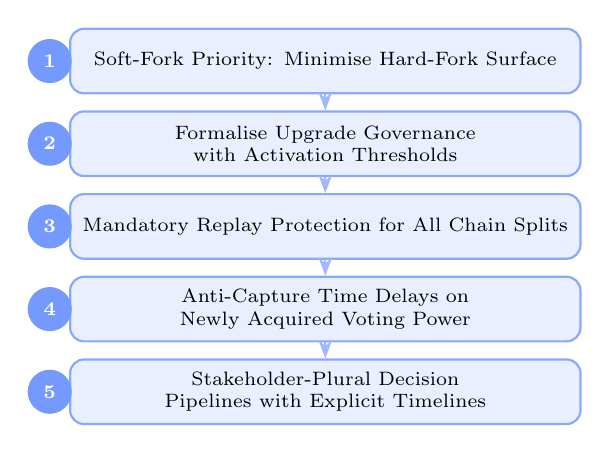
\begin{tikzpicture}[
  font=\scriptsize,
  >=Stealth,
  pbox/.style={
    rectangle, rounded corners=5pt,
    minimum width=6.4cm, minimum height=0.82cm,
    draw=accentblue!55, thick,
    fill=accentblue!10, text centered,
    text width=6.2cm, align=center, inner sep=4pt
  },
  num/.style={
    circle, fill=accentblue!65, text=white,
    minimum size=0.56cm,
    font=\bfseries\scriptsize
  },
  arr/.style={-{Stealth}, thick, accentblue!45}
]

  \node[pbox] (p1) at (0.25, 0.0)  {Soft-Fork Priority: Minimise Hard-Fork Surface};
  \node[pbox] (p2) at (0.25,-1.05) {Formalise Upgrade Governance with Activation Thresholds};
  \node[pbox] (p3) at (0.25,-2.10) {Mandatory Replay Protection for All Chain Splits};
  \node[pbox] (p4) at (0.25,-3.15) {Anti-Capture Time Delays on Newly Acquired Voting Power};
  \node[pbox] (p5) at (0.25,-4.20) {Stakeholder-Plural Decision Pipelines with Explicit Timelines};

  \node[num] at (-3.25, 0.0)  {1};
  \node[num] at (-3.25,-1.05) {2};
  \node[num] at (-3.25,-2.10) {3};
  \node[num] at (-3.25,-3.15) {4};
  \node[num] at (-3.25,-4.20) {5};

  \draw[arr] (p1.south) -- (p2.north);
  \draw[arr] (p2.south) -- (p3.north);
  \draw[arr] (p3.south) -- (p4.north);
  \draw[arr] (p4.south) -- (p5.north);

\end{tikzpicture}
\caption{Five design principles for reducing governance-driven forks, ordered from
  technical-layer to coordination-layer applicability.}
\label{fig:principles}
\end{figure}

{\raggedright
\textbf{Principle 1 --- Soft-Fork Priority.}
Backward-compatible changes lower the probability of splits because non-upgraded nodes
remain on the same chain~\cite{bip9,bitcoincore-versionbits}.

\textbf{Principle 2 --- Formalise Upgrade Governance.}
Tezos uses on-chain proposals and protocol votes~\cite{tezos-governance}; Polkadot's
forkless runtime upgrades~\cite{polkadot-runtimeupgrades} achieve a similar effect.
Hybrid governance---open off-chain deliberation combined with narrow on-chain
signaling---mitigates stake-concentration risk.

\textbf{Principle 3 --- Mandatory Replay Protection.}
EIP-155~\cite{eip155} and Bitcoin Cash's \texttt{SIGHASH\_FORKID}~\cite{uahf-spec}
demonstrate that replay protection should be a baseline safety rail, enabling peaceful
chain coexistence.

\textbf{Principle 4 --- Anti-Capture Time Delays.}
Hive introduced a 30-day delay before newly staked tokens could vote~\cite{hive-launch}.
Cardano's Voltaire adds constitutional committee oversight~\cite{cardano-voltaire2024}.
Time delays prevent sudden mobilization via custodial exchanges or market purchases.

\textbf{Principle 5 --- Stakeholder-Plural Decision Pipelines.}
BIP-2 argues that hard-fork adoption requires the broader Bitcoin economy~\cite{bip2}.
Ethereum's EIP-1 explicitly acknowledges dissent as normal~\cite{ethereum-eip1}.
Transparent pipelines with explicit timelines and multi-class activation thresholds
reduce incentives for ``surprise forks'' driven by distrust.

%%──────────────────────────────────────────────────────────────────────────────
\section{Limitations and Future Work}
%%──────────────────────────────────────────────────────────────────────────────

Fork frequency data (Figure~\ref{fig:fork-freq}) relies on publicly reported events and
market capitalization thresholds; smaller forks are undercounted. The causal claim that
governance design \emph{reduces} forks is not established by observational data alone.
Future work should examine: (1)~Cardano's Voltaire rollout outcomes~\cite{cardano-voltaire2024};
(2)~whether Ethereum's validator-set governance produces capture risks analogous to DPoS;
(3)~empirical analysis of anti-capture time delays; and (4)~cross-chain governance
interactions as IBC and bridging create inter-governance dependencies.

%%──────────────────────────────────────────────────────────────────────────────
\section{Conclusion}
%%──────────────────────────────────────────────────────────────────────────────

Governance-driven hard forks are sociotechnical events whose outcomes depend on technical
architecture, coordination mechanisms, and legitimacy dynamics in ways that cannot be
reduced to any single dimension. Our analysis of three canonical cases and a twelve-network
taxonomy reveals that the most effective governance models combine hybrid on-chain/off-chain
coordination, mandatory replay protection, and anti-capture safeguards. The empirical trend
toward fewer contentious forks among mature networks after 2020 correlates with the adoption
of precisely these features.

The right to fork is not a failure mode to be engineered away. It is the mechanism by which
dissenting communities can exit without institutional permission, and the credible threat
that keeps informal power holders accountable. The design challenge is to make the
\emph{exercise} of that right rare, safe, and orderly---not to make it impossible.

%%──────────────────────────────────────────────────────────────────────────────
\sloppy
\bibliographystyle{ACM-Reference-Format}
\begin{thebibliography}{99}

\bibitem{nakamoto2008bitcoin}
S.~Nakamoto, ``Bitcoin: A Peer-to-Peer Electronic Cash System,'' 2008.
\url{https://bitcoin.org/bitcoin.pdf}

\bibitem{buterin2014ethereum}
V.~Buterin, ``A Next-Generation Smart Contract and Decentralized Application Platform,''
\emph{Ethereum White Paper}, 2014.

\bibitem{atzei2017survey}
N.~Atzei, M.~Bartoletti, and T.~Cimoli, ``A Survey of Attacks on Ethereum Smart
Contracts,'' \emph{Proc.\ POST}, 2017.

\bibitem{walch2019code}
A.~Walch, ``In Code(rs) We Trust,'' \emph{Regulating Blockchain}, Oxford University
Press, 2019.

\bibitem{de2021blockchain}
F.~De Filippi, P.~Mannan, and W.~Reijers, ``Blockchain as a Confidence Machine,''
\emph{Technology in Society}, vol.~64, 2021.

\bibitem{reijers2021governance}
W.~Reijers et al., ``Now the Code Runs Itself,'' \emph{Topoi}, vol.~40,
pp.~821--831, 2021.

\bibitem{beck2018governance}
R.~Beck, C.~Müller-Bloch, and J.~King, ``Governance in the Blockchain Economy,''
\emph{Journal of the AIS}, vol.~19, no.~10, 2018.

\bibitem{tan2020blockchain}
L.~Tan et al., ``Blockchain Governance: A Literature Review,'' \emph{IEEE Access},
vol.~8, 2020.

\bibitem{lumineau2021blockchain}
F.~Lumineau, W.~Wang, and O.~Schilke, ``Blockchain Governance,''
\emph{Organization Science}, vol.~32, no.~2, pp.~500--521, 2021.

\bibitem{el-amine2022}
H.~El-Amine et al., ``Decentralized Governance in Blockchain Ecosystems,''
\emph{Proc.\ ACM WebSci}, 2022.

\bibitem{multistakeholder2023}
T.~Behnke and J.~Ritter, ``Multi-Stakeholder Governance Lessons from the Hive Fork,''
\emph{Ledger}, vol.~8, 2023.

\bibitem{judmayer2017merged}
A.~Judmayer et al., ``Merged Mining: Curse or Cure?,'' \emph{DPM/CBT}, 2017.

\bibitem{eskandari2021sok}
S.~Eskandari et al., ``SoK: Diving into DAOs,'' \emph{Proc.\ IEEE S\&B}, 2021.

\bibitem{liu2021fork}
Z.~Liu et al., ``A Survey on Applications of Game Theory in Blockchain,''
\emph{IEEE Commun.\ Surveys Tut.}, 2021.

\bibitem{biais2019blockchain}
B.~Biais et al., ``The Blockchain Folk Theorem,'' \emph{Rev.\ Financial Studies},
vol.~32, no.~5, pp.~1662--1715, 2019.

\bibitem{gencer2018decentralization}
A.~E.~Gencer et al., ``Decentralization in Bitcoin and Ethereum Networks,''
\emph{Proc.\ FC}, 2018.

\bibitem{sec2017dao}
U.S.\ Securities and Exchange Commission, ``Report of Investigation: The DAO,''
Release No.~81207, July 2017.
\url{https://www.sec.gov/files/litigation/investreport/34-81207.pdf}

\bibitem{eth-hardfork2016}
Ethereum Foundation, ``Hard Fork Completed,'' July 2016.
\url{https://blog.ethereum.org/2016/07/20/hard-fork-completed}

\bibitem{eip779}
``EIP-779: Hardfork Meta: DAO Fork.''
\url{https://eips.ethereum.org/EIPS/eip-779}

\bibitem{eip155}
``EIP-155: Simple Replay Attack Protection.''
\url{https://eips.ethereum.org/EIPS/eip-155}

\bibitem{eip1}
``EIP-1: EIP Purpose and Guidelines.''
\url{https://eips.ethereum.org/EIPS/eip-1}

\bibitem{ethereum-eip1}
``EIP-1: EIP Purpose and Guidelines.''
\url{https://eips.ethereum.org/EIPS/eip-1}

\bibitem{etc-codeislaw}
Ethereum Classic, ``Code is Law.''
\url{https://ethereumclassic.org/why-classic/code-is-law/}

\bibitem{ethereum-merge2022}
Ethereum Foundation, ``The Merge,'' September 2022.
\url{https://ethereum.org/en/upgrades/merge/}

\bibitem{bitcoin-bips}
Bitcoin BIPs Repository. \url{https://github.com/bitcoin/bips}

\bibitem{bip2}
``BIP-2: BIP Process, Revised.'' \url{https://bips.dev/2/}

\bibitem{bip9}
``BIP-9: Version Bits with Timeout and Delay.'' \url{https://bips.dev/9/}

\bibitem{bip141}
``BIP-141: Segregated Witness (Consensus Layer).'' \url{https://bips.dev/141/}

\bibitem{bip148}
``BIP-148: Mandatory Activation of SegWit Deployment.'' \url{https://bips.dev/148/}

\bibitem{bitcoincore-versionbits}
Bitcoin Core, ``Version Bits BIP9 FAQ,'' June 2016.
\url{https://bitcoincore.org/en/2016/06/08/version-bits-miners-faq/}

\bibitem{dcg-nya}
Digital Currency Group, ``Bitcoin Scaling Agreement at Consensus 2017,'' 2017.
\url{https://dcgco.medium.com/bitcoin-scaling-agreement-at-consensus-2017-133521fe9a77}

\bibitem{fed-bitcoin2019}
Federal Reserve Bank of Cleveland, ``Bitcoin's Decentralized Decision Structure,''
\emph{Economic Commentary}, 2019.

\bibitem{uahf-spec}
Bitcoin Cash Node, ``UAHF Technical Specification,'' v1.6, 2017.
\url{https://upgradespecs.bitcoincashnode.org/uahf-technical-spec/}

\bibitem{binance-dpos}
Binance Academy, ``Delegated Proof of Stake Explained.''
\url{https://www.binance.com/en/academy/articles/delegated-proof-of-stake-explained}

\bibitem{knight-steemit}
Knight First Amendment Institute, ``Crypto Logic Platforms and Steemit,'' Oct.\ 2020.
\url{https://knightcolumbia.org/blog/}

\bibitem{hive-launch}
Hive.blog, ``Announcing the Launch of Hive Blockchain,'' March 20, 2020.
\url{https://hive.blog/communityfork/@hiveio/announcing-the-launch-of-hive-blockchain}

\bibitem{binance-governance-policy2020}
Binance, ``Clarification on Steem Governance Vote,'' March 2020.
\url{https://www.binance.com/en/blog/community/clarification-on-steem-governance-vote}

\bibitem{tezos-governance}
Tezos Documentation, ``Governance and Self-Amendment.''
\url{https://docs.tezos.com/architecture/governance}

\bibitem{polkadot-runtimeupgrades}
Polkadot Wiki, ``Runtime Upgrades.''
\url{https://wiki.polkadot.com/learn/learn-runtime-upgrades/}

\bibitem{cardano-voltaire2024}
Cardano Foundation, ``Voltaire Governance Rollout,'' 2024.
\url{https://cardano.org/governance/}

\bibitem{coinmarketcap2024}
CoinMarketCap, ``Ethereum Classic (ETC) Market Data,'' 2024.
\url{https://coinmarketcap.com/currencies/ethereum-classic/}

\bibitem{werbach2018trust}
K.~Werbach, ``The Trustless Machine,''
\emph{Colorado Technology Law Journal}, vol.~16, no.~1, 2018.

\bibitem{wright2015decentralized}
A.~Wright and P.~De Filippi, ``Decentralized Blockchain Technology and the Rise of
Lex Cryptographia,'' 2015.

\end{thebibliography}

\end{document}
